\newpage
\section{Example: Microwave Oven}
\label{microwave}
\begin{figure}[!t]
\centering
\includegraphics[width=0.75\textwidth]{../images/microwave.png}
\caption{A state-machine diagram for the microwave oven}
\label{fig_microwave}
\end{figure}

For the next case study, we examine the classic and well-known {\em
  microwave oven} problem.  In essence, we have a microwave oven with
a door and a heating element.  An important safety condition is that
the heating element cannot be on when the door is open, to protect
against burns.  This example is interesting, because it demonstrates
that Whiley can operate effectively as a modelling language, as well
as a general-purpose programming language.

\subsection{Overview}
Figure~\ref{fig_microwave} provides a state-machine diagram of the
microwave oven.  The microwave state has three components: a heating
element, which is set either {\em on} or {\em off}; a door which (via
a sensor) is recorded as either {\em open} or {\em closed}; and, finally, a timer value indicating how for many seconds heating should occur.

In addition to the microwave state, a number of external events are permitted.  First, a start button is used to signal the microwave should begin heating; second, the door may be opened or closed; finally, an internal clock is used to signal time passing (in one second intervals) to the state machine.

\subsection{Microwave State}
The state of the microwave is represented in Whiley using a record containing the main three components, along with an appropriate invariant.  The following illustrates:

\lstinputlisting[firstline=7,lastline=14]{../examples/microwave.whiley}

Here, boolean values are used to represent the state of the heating element, and the door sensor, whilst a natural number represents the timer value.  The invariant states that either the door is closed, or the heating element is off.

\subsection{Events}

Events can be modelled in Whiley using functions which map one microwave state to another.  Here are the two functions representing the {\em open} and {\em close} events:

\lstinputlisting[firstline=47,lastline=60]{../examples/microwave.whiley}

Here, we can see that preconditions on the functions act as guards restricting when the events may fire.  The Whiley compiler will statically verify that the \lstinline{Microwave} invariant holds for the turn value, assuming it held for the parameter.  Thus, failing to set \lstinline{m.heatOn = false} in \lstinline{doorOpened()} results in a compile time error which signal that the safety property is not be enforced.

Likewise, we can specify the {\em start} event and, in doing so, we must ensure the safety property is enforced.  Specifically, when the heating element is turned on, the door must be closed:

\lstinputlisting[firstline=38,lastline=45]{../examples/microwave.whiley}

Here we can see that, if the door is open when the start button is pressed, nothing happens.  Again, failing to check whether the door is open in \lstinline{startCooking()} results in a compile time error which signal that the safety property is not be enforced.
